    %%%%%%%%%%%%%%%%%%%%%%%%%%%%%%%%%%%%%%%%%%%%%%%%%%%%%%%%%%%%%%%%%%%%%%%%%%%%%%%%%%%%
% Do not alter this block (unless you're familiar with LaTeX)
\documentclass{../labbook}
%%%%%%%%%%%%%%%%%%%%%%%%%%%%%%%%%%%%%%%%%%%%%
%Fill in the appropriate information below
\lhead{Cantao Su}
\rhead{Speech Sounds} 
\chead{\textbf{Lab Book A4. Due: 11.10.2023 23:59 CEST}}
%%%%%%%%%%%%%%%%%%%%%%%%%%%%%%%%%%%%%%%%%%%%%

\begin{document}

\begin{mdframed}[backgroundcolor=blue!20]
\LaTeX~submissions are mandatory. Submitting your assignment in another format will be graded no higher than R. Convenient table for the TIPA package used to processing IPA symbols can be found \href{https://jon.dehdari.org/tutorials/tipachart_mod.pdf}{here}. Detailed TIPA manual can be found \href{http://www.l.u-tokyo.ac.jp/~fkr/tipa/tipaman.pdf}{here}.
\end{mdframed}

\tableofcontents %Automatic table of contents

\section{Lab Book A4.}
In Lab Book A4 we are focusing on the vowel formants. We will be able to see the formant tracks over time. To examine these things we are going to use \href{https://www.fon.hum.uva.nl/praat/}{Praat} and the programming language of your choice.
This Lab Book partly follows the tutorial of Matthew Winn, you can watch his instructions for Praat and R in his \href{https://youtu.be/BGW8J4cG0qY}{youtube video}.

\subsection{Submission}
For this submission you will need to commit the {\LaTeX} file as usual, as well as one picture as part of the task 1 (both the LaTeX file and picture(s) should be committed to A4 folder in your GitHub repository). 

\begin{problem}{1}{10}{Formant tracks}

\subsubsection*{Preparation:}

Record yourself speaking the ``hVd'' words (quiet environment, .wav foramt, sampling rate 44.1kHz). Below is the list of these words. Typical F1-F3 formant values are provided for 8 vowels as calculated for AmE (Ladefoged \& Johnson, 2015).

\begin{tabular}{lll}
heed   &\textipa{/hi:d/} 
    & $F_1$ = 280 Hz, $F_2$ = 2250 Hz, $F_3$ = 2890 Hz \\ 
hid    &\textipa{/hId/} 
    & $F_1$ = 400 Hz, $F_2$ = 1920 Hz, $F_3$ = 2560 Hz   \\ 
hayed  &\textipa{/heId/}   \\ 
head   &\textipa{/hEd/}
    & $F_1$ = 550 Hz, $F_2$ = 1770 Hz, $F_3$ = 2490 Hz \\ 
had    &\textipa{/h\ae d/}
    & $F_1$ = 690 Hz, $F_2$ = 1660 Hz, $F_3$ = 2490 Hz \\ 
hod    &\textipa{/h6d/} (can \textipa{/hAd/})
    & $F_1$ = 710 Hz, $F_2$ = 1100 Hz, $F_3$ = 2540 Hz  (\textipa{/A/})\\ 
hawed  &\textipa{/hOd/}
    & $F_1$ = 590 Hz, $F_2$ = 880 Hz, $F_3$ = 2540 Hz \\ 
hud    &\textipa{/h2d/}    \\ 
hoed   &\textipa{/hoUd/}   \\ 
hood   &\textipa{/hUd/} 
    & $F_1$ = 450 Hz, $F_2$ = 1030 Hz, $F_3$ = 2380 Hz \\ 
who'd  &\textipa{/hud/} 
    & $F_1$ = 310 Hz, $F_2$ = 870 Hz, $F_3$ = 2250 Hz  \\ 
how'd  &\textipa{/haUd/}   \\ 
hoyed  &\textipa{/hOId/}   \\ 
hide   &\textipa{/hAId/} (can be \textipa{/h2Id/} or \textipa{/haId/}) \\ 
height &\textipa{/hAIt/} (can be \textipa{/h2It/} or \textipa{/haIt/}) \\ 
herd   &\textipa{/h3(r)d/} \\ 
ahead  &\textipa{/@hEd/} (here we are interested in schwa!)
\end{tabular}

Next, annotate the vowels in those words using TIPA or the same two-letter sequences that Matthew Winn suggests in his video. \textbf{Hint}: instead of annotating the whole vowel you can annotate the stable part of the vowel to make the formant tracks even be cleaner. You can do it by placing boundaries several periods into the vowel and several periods before the vowel's end.

Using Matt's formant script (available \href{https://github.com/ListenLab/make_vowel_space/blob/main/Extract_formants.txt}{here}), extract the table of formants for all the vowels. Make sure to tune the parameters in the script to get at least 10 measurements of each of three formants, and don't forget to configure the formant tracker in Praat: inaccurate formant settings lead to inaccurate formant chart. In the script above there is no form and no path needed: you will work with a sound file and a TextGrid that you open in your Praat. Follow instructions in the script and in the video.

Save this table as comma-separated file if you are working with R code and as white space separated with Python code. This will be the input data for the task.

\subsubsection*{Task:}
\begin{itemize}
    \item If you are working with R use the script provided \href{https://github.com/ListenLab/make_vowel_space/blob/main/Plot_vowel_space.R}{here}. If you are working with Python use the script provided \href{https://github.com/Equidamoid/vowel_space_plot}{here}\footnote{The Python script differs from R script,  the mapping of the vowel labels to IPA Unicode symbols is not done there. Feel free to do it yourself if you want to: all the Unicode symbols for vowels can be found on Wikipedia: \href{https://en.wikipedia.org/wiki/Phonetic_symbols_in_Unicode\#Vowels}{here}.}. You are also allowed to in any other programming language.
    
    \item Using this script to plot the tracks of your vowels' formants. You will see how the formant values change within one vowel. If you do not have the IPA labels on your plot, provide the mapping in your solution (e.g., ``ii'' = [i]).
    
    \item Include the image of your plot in your answer. Below is an example showing how to include a picture in a LaTeX document. 

    \item Examine the formant tracks of your vowels. Describe the dynamic patterns you see:
    \begin{itemize}
        \item How do your front vowels move? (describe at least two)
        \item How do your back vowels move? (describe at least two)
        \item How do your diphthongs move? (describe at least two)
        \item Where do your central vowels start?
        \item Is there a difference for your diphthongs in ``height'' and ``hide''? 
    \end{itemize} 
   
\end{itemize}

\end{problem}

    \begin{figure}[h!]
        \centering
        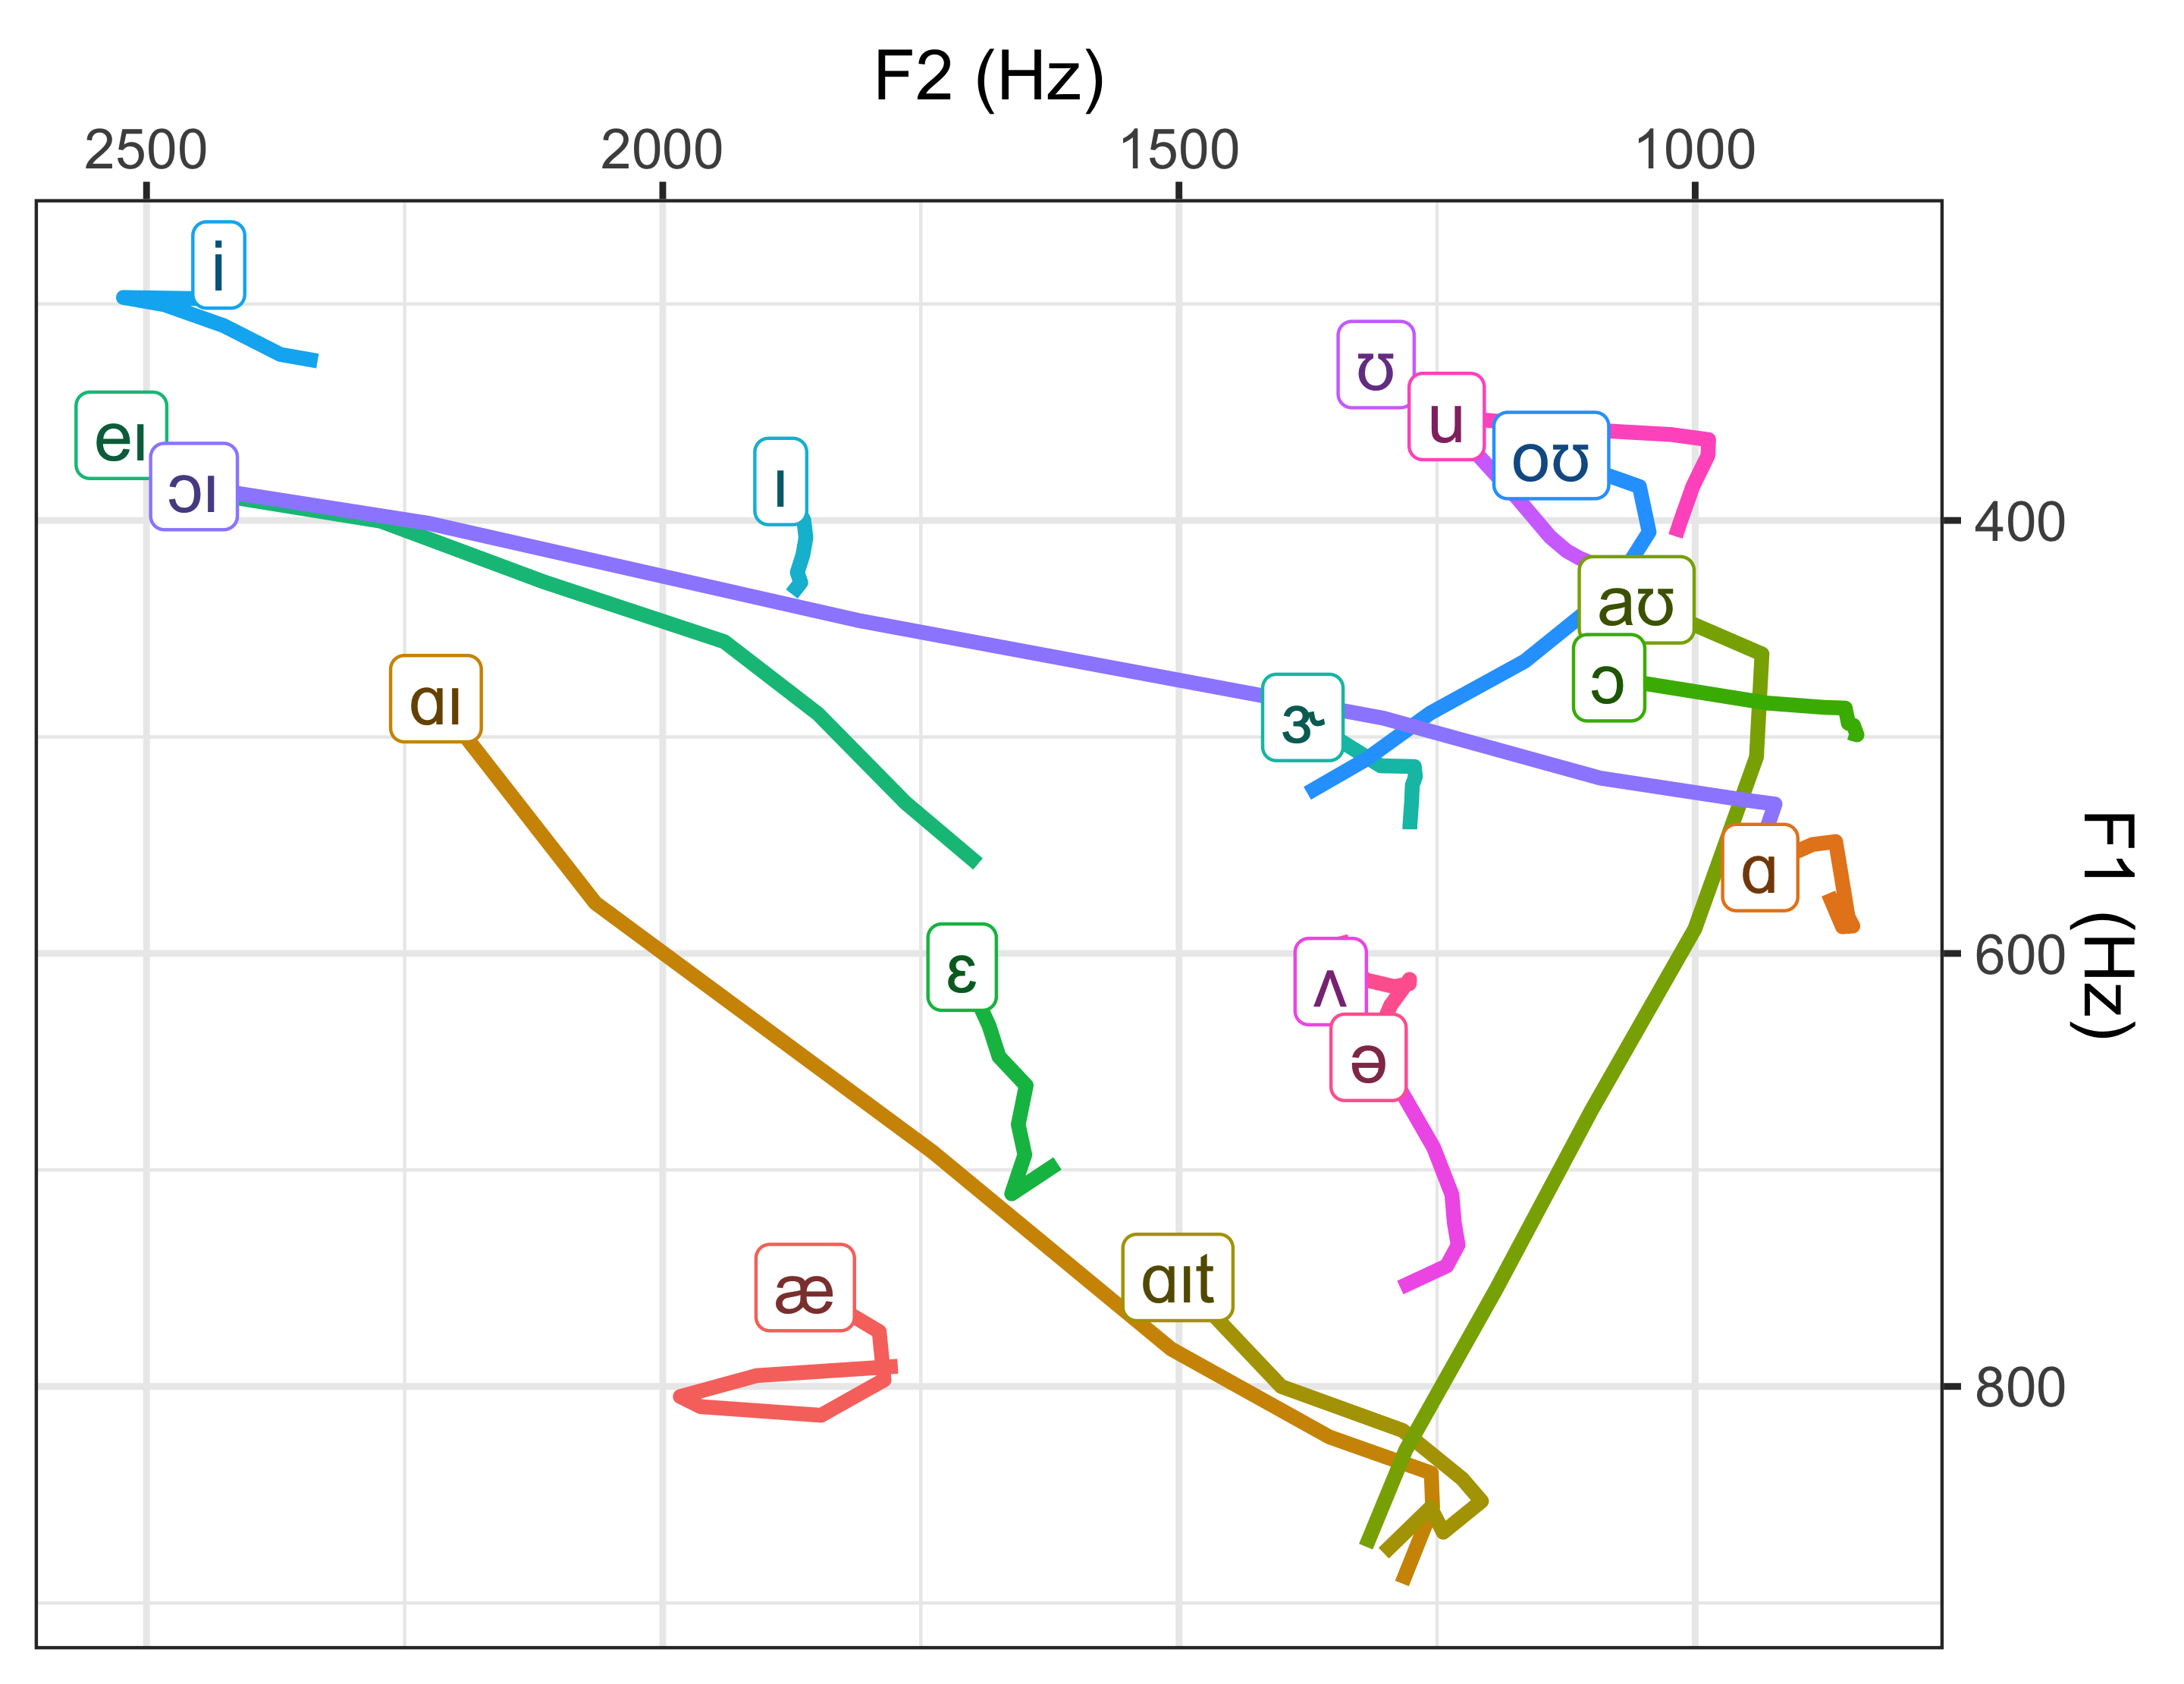
\includegraphics[width=0.69\textwidth]{Cantao Su_Track of Vowel's Formants.jpg}
        \caption{Tracks of Vowels' Formants}
	\end{figure}

    

%%%%%%%%%%%%%%%%%%%%%%%%%%%%%%%%%%%%%%%%%%%%%
\begin{solution}
\begin{itemize}
    \item Movement of front vowels
    \begin{enumerate}
        \item /i/: slightly lower F1 but higher F2 concurrently, with the tongue higer and more forward.
        \item /\ae/: basically unchanged with both F1 and F2 slightly fluctuating but turning back to almost the original point.
    \end{enumerate}
    \item Movement of back vowels
    \begin{enumerate}
        \item /u/: lower F1 and then higher F2 sequently ,with the tongue higer and more forward.
        \item /\textopeno/: slightly lower F1 but higher F2 concurrently, with the tongue higer and more forward.
    \end{enumerate}
    \item Movement of diphtongs 
    \begin{enumerate}
        \item /\textscripta \textsci /: dramatically lower F1 but higher F2 concurrently, with the tongue higer and more forward.
        \item /a\textupsilon /: dramatically lower F1 and F2 but then slightly higher F2, with tongue generally higher and more backward.  
    \end{enumerate}
    \item Initial places of central vowels 
    \begin{enumerate}
        \item /\textrhookschwa /: center-back and middle (at around F1 of 540Hz and F2 of 1280Hz)
        \item /\textschwa /: center-back but low, even approaching open vowels (at around F1 of 750Hz and F2 of 1300Hz)
    \end{enumerate}
    \item Differences between \textscripta \textsci / in ``height'' and ``hide''
    \begin{enumerate}
        \item much longer duration of the diphthong in ``height'' than ``hide''
        \item more dramatic decrease of F1 and increase of F2 of the diphthong in ``height'' than ``hide''
    \end{enumerate}
\end{itemize}
\end{solution}
%%%%%%%%%%%%%%%%%%%%%%%%%%%%%%%%%%%%%%%%%%%%%


\bigskip
\textbf{References}:

\noindent Ladefoged, P., \& Johnson, K. (2015). A course in phonetics. Cengage learning.

Liu, H. M., Tsao, F. M., \& Kuhl, P. K. (2005). The effect of reduced vowel working space on speech intelligibility in Mandarin-speaking young adults with cerebral palsy. The Journal of the Acoustical Society of America, 117(6), 3879-3889.

Roy, N., Nissen, S. L., Dromey, C., \& Sapir, S. (2009). Articulatory changes in muscle tension dysphonia: Evidence of vowel space expansion following manual circumlaryngeal therapy. Journal of communication disorders, 42(2), 124-135.


\end{document}


